\documentclass{article}
\title{MATH 2400 HW0}
\author{Xinshi,Wang}
\usepackage[letterpaper,textwidth=5.5in,right=0.6in,textheight=9in,left=0.6in,top=0.7in,bottom=0.7in]{geometry}
\usepackage{scrextend}
\usepackage{graphicx}
\usepackage{xcolor}
\usepackage{amssymb}
\usepackage{amsmath}
\usepackage{setspace}
\begin{document}
	\noindent
	MATH 2400 HW0 \\
	Wang Xinshi\\
	
	1.$I_a = \int x \ln x \,dx$
	\begin{align*}
		&\int x \ln x \,dx\\
		&=\dfrac{lnx}{2}x^2-\int\dfrac{x^2}{2}\dfrac{1}{x}+C\\
		&=\dfrac{lnx}{2}x^2-\int \dfrac{x}{2}+C\\
		&=\dfrac{lnx}{2}x^2-\dfrac{x^2}{4}+C
	\end{align*}

    2.$I_b = \int \dfrac{x}{x^2+3} \,dx$
    \begin{align*}
    	&\int \dfrac{x}{x^2+3} \,dx\\
    	&\text{Let $u = x^2+3$, then $\,du = 2x \,dx$}\\
    	&=\dfrac{1}{2} \int \dfrac{1}{u} \,du+C\\
    	&=\dfrac{1}{2} \ln u +C\\
    	&=\dfrac{1}{2} \ln(x^2+3)+C
    \end{align*}
	
	3.$I_c = \int_{0}^{2} te^{-t} \,dt$
	\begin{align*}
		&\int_{0}^{2} te^{-t} \,dt\\
		&=-te^{-t}\Big|_0^2+ \int_{0}^{2} e^{-t}dt\\
		&=-2e^{-2}-e^{-t} \Big|_0^2\\
		&=1-3e^{-2}\\
	\end{align*}

	4.$y^2+2y+t^3+sin(t)-3 = 0$
	\begin{align*}
		y^2+2y+t^3+sin(t)-3&= 0\\
		y^2+2y&=3-sin(t)-t^3\\
		y^2+2y+1&=4-sin(t)-t^3\\
		(y+1)^2&=4-sin(t)-t^3 \\
		y&=\\sqrt{4-sin(t)-t^3}-1
	\end{align*}
	\newpage

	5.\\
		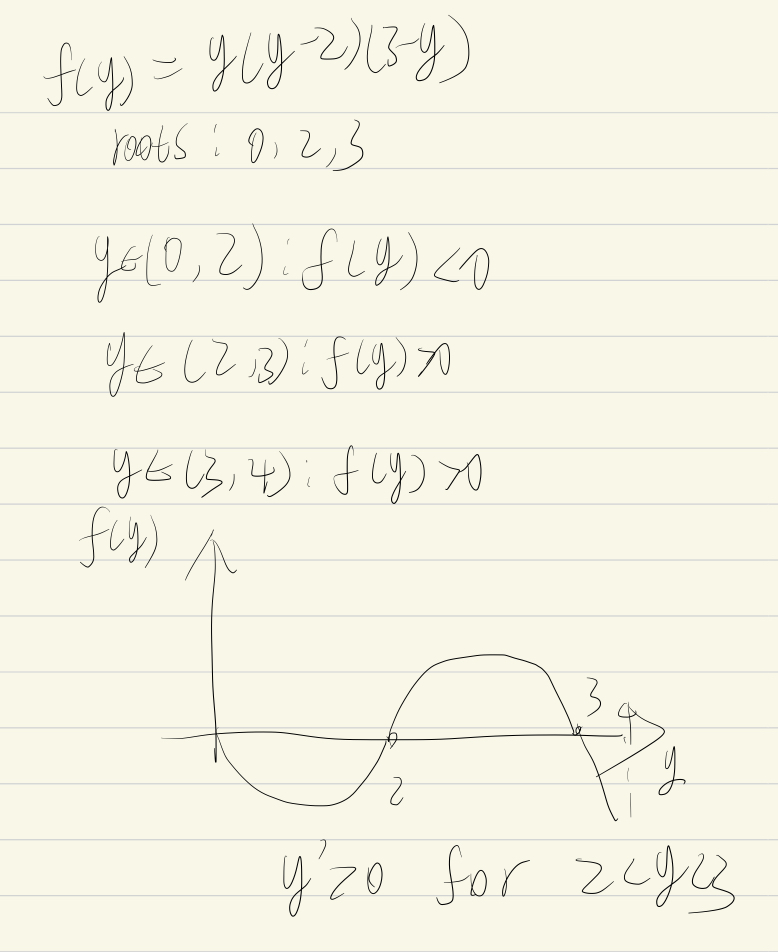
\includegraphics[scale = 0.3]{"C:/Users/Micha/OneDrive - Rensselaer Polytechnic Institute/MATH2400/pictures/p5.jpg"}

\end{document} 